% AUTO-GENERATED by scripts/gen_tables.py -- do not hand-edit.
\begin{figure}[t]
\centering
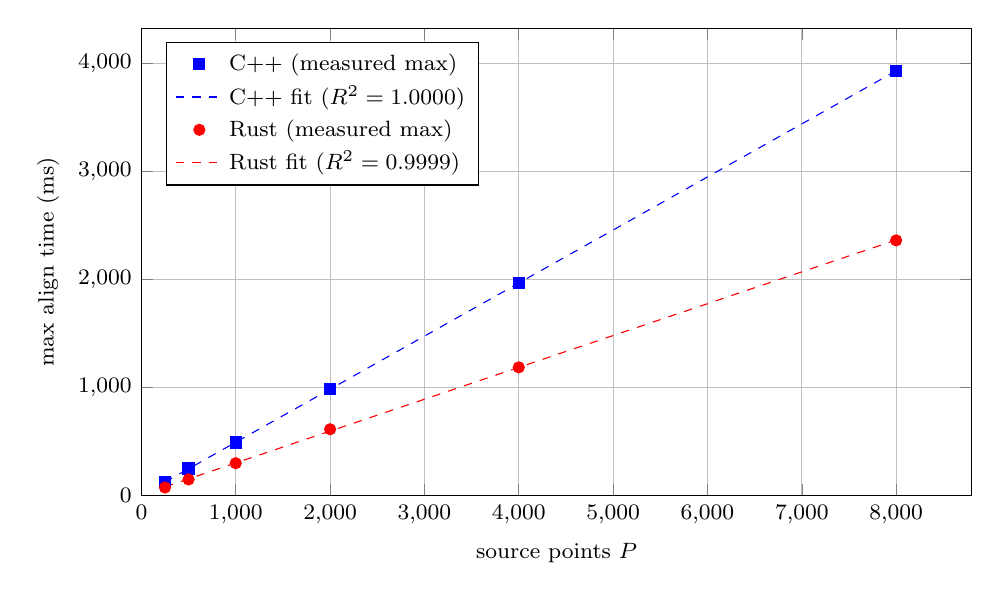
\begin{tikzpicture}
\begin{axis}[
  width=\columnwidth, height=0.62\columnwidth,
  xlabel={source points $P$}, ylabel={max align time (ms)},
  xmin=0, ymin=0, legend pos=north west, legend cell align=left,
  grid=major, tick label style={font=\footnotesize}, label style={font=\footnotesize},
  legend style={font=\footnotesize},
]
\addplot[only marks, mark=square*, color=blue] coordinates { (250,126.34) (500,251.75) (1000,491.65) (2000,982.99) (4000,1964.51) (8000,3930.39) };
\addlegendentry{C++ (measured max)}
\addplot[no marks, color=blue, dashed] coordinates { (250,125.68) (8000,3929.18) };
\addlegendentry{C++ fit ($R^2=1.0000$)}
\addplot[only marks, mark=*, color=red] coordinates { (250,75.07) (500,149.78) (1000,300.09) (2000,613.89) (4000,1186.54) (8000,2361.07) };
\addlegendentry{Rust (measured max)}
\addplot[no marks, color=red, dashed] coordinates { (250,81.34) (8000,2364.69) };
\addlegendentry{Rust fit ($R^2=0.9999$)}
\end{axis}
\end{tikzpicture}
\caption{Observed maximum align latency vs.\ source-point count $P$ on the
Rust-search geometry
(common kernel evaluations per point held invariant; traversal counters measured separately).
Dashed lines are descriptive affine fits
through the six observed maxima, not hard latency bounds.}
\label{fig:psweep}
\end{figure}
